\section{Introduction}

In this contribution, we introduce SuperMat (Superconductor Materials), an annotated corpus of linked data derived from scientific publications on superconductors, which comprises 164 articles, 18698 entities, and 1524 links that are characterised into two layers. The first layer contains six categories: the names, classes, and properties of materials; links to their respective superconducting critical temperature (\tc); and parametric conditions such as applied pressure or measurement methods.
The second layer is dedicated to material entities and contains eight classes: formula, name, doping ratio, etc. 
The construction of SuperMat resulted from a fruitful collaboration between computer scientists and material scientists, and its high quality is ensured through validation by domain experts. 
The quality of the annotation guidelines was ensured by a satisfactory Inter Annotator Agreement (IAA) between the different annotators. 
SuperMat includes the dataset, annotation guidelines, and annotation support tools that use automatic suggestions to help minimise human errors.

\label{content-acquisition}
\section{Content acquisition}
SuperMat originates from PDF documents of scientific articles related to superconductor research. 
The original documents were collected from the following sources: (a) the Open Access (OA) version of peer-reviewed articles referenced in the SuperCon database records; 
(b) articles provided by domain experts containing suitable items and potential links of material names, \tc~values, measurement methods, and pressures; (c) articles from "condensed matter" category of arXiv (\url{https://arxiv.org/archive/cond-mat}) selected using the search terms of "superconductor", "critical temperature", and "superconductivity". 

Pre-print versions of peer reviewed articles were obtained using a bibliographic data lookup service called biblio-glutton (\url{https://github.com/kermitt2/biblio-glutton}) that aggregates data from various sources: the Crossref (\url{https://www.crossref.org/}) bibliographic database, the unPaywall (\url{http://unpaywall.org}) service, the PubMed Central repository (\url{https://pubmed.ncbi.nlm.nih.gov/}), and mappings to other databases. 
We queried \textit{biblio-glutton} using the bibliographic data of each article referenced in Supercon; subsequently, we downloaded the pre-print article associated with the retrieved record, if available. 
Although the published version may differ from the pre-print version of a document, the differences measured by comparing pre-print and peer-reviewed articles in biology~\cite{carneiro_comparing_2020} measured objective differences to be around 5\% %.


\section{Preliminary annotation study}
\label{subsec:preliminary-annotation-study}
A preliminary annotation study was carried out to assess the effort required from the annotators to reach an acceptable Inter Annotation Agreement (IAA \textgreater 0.7) .
We annotated two randomly selected OA papers, by using a preliminary version of the guidelines with a limited tag-set of four labels: \texttt{<material>}, \texttt{<tc>} (expression describing the presence or absence of superconductivity), \texttt{<tcValue>} (value of \tc), and \texttt{<doping>} (amount of substitution, such as stochiometric values, usually expressed as functions of x or y).
The process was iterated multiple times.
Each iteration ended with computing the IAA using the Krippendorff's alpha coefficient~\cite{Krippendorff2004ReliabilityIC,Zapf2016MeasuringIR}, while annotators discussed the disagreements, and updated the guidelines.

\begin{table}[htbp]
    \centering
    \caption{Summary of the IAA for each annotation iteration.}
    \begin{tabular}{ ccc } 
    \toprule
        \textbf{Iteration} \# & \textbf{IAA} & \textbf{IAA by label}  \\ [0.5ex] 
    \midrule
        1  & 0.45
        &\begin{tabular}{  cc  } 
            \texttt{<material>} & 0.45\\ 
            \texttt{<tc>} & 0.56\\
            \texttt{<tcValue>} & 0.50\\
            \texttt{<doping>} & 0.21\\
        \end{tabular}    
        \\ 
    \midrule
        2 & 0.65
        &\begin{tabular}{  cc  } 
            \texttt{<material>} & 0.75\\ 
            \texttt{<tc>} & 0.85\\
            \texttt{<tcValue>} & 0.85\\
            \texttt{<doping>} & 0.39 \\
        \end{tabular}          
        \\ 
    \midrule
        3 & 0.89
        & \begin{tabular}{  cc  } 
            \texttt{<material>} & 0.89\\ 
            \texttt{<tc>} & 0.91\\
            \texttt{<tcValue>} & 0.88\\
            \texttt{<doping>} & 0.94\\
        \end{tabular}       
        \\ 
    \bottomrule
    \end{tabular}
    
    \label{table:summary-preliminary-annotation}
\end{table}

Based on the results in Table~\ref{table:summary-preliminary-annotation}, IAA reached a satisfactory level of around 0.9 after the third iteration. 
Although the average IAA reached 0.7 on three of the four labels in the second iteration, the average agreement was unsatisfactory. 
When analysing the disagreement, we noticed that the low score in the \texttt{<doping>} label was caused by a heavy overlap with the \texttt{<material>} label, which required a more precise definition in the guidelines. 

Based on this preliminary study, the following changes were implemented. 
(a) The label \texttt{<doping>} was merged under the \texttt{<material>} because, even with detailed documentation it was too difficult for humans to annotate them consistently.
(b) Three more labels were added: measurement methods and pressure (described as parametric conditions in relation to \tc), and class of materials. 

\section{Tag-set design}
The tag set (also referred to as \textit{labels}) represents the classes of entities and the type of links between them, which were designed to be extracted from the text (Figure~\ref{fig:example-annotations-and-links}).

% example-annotated-corpus-postprocess.png
\begin{figure}[htbp]
  \centering
  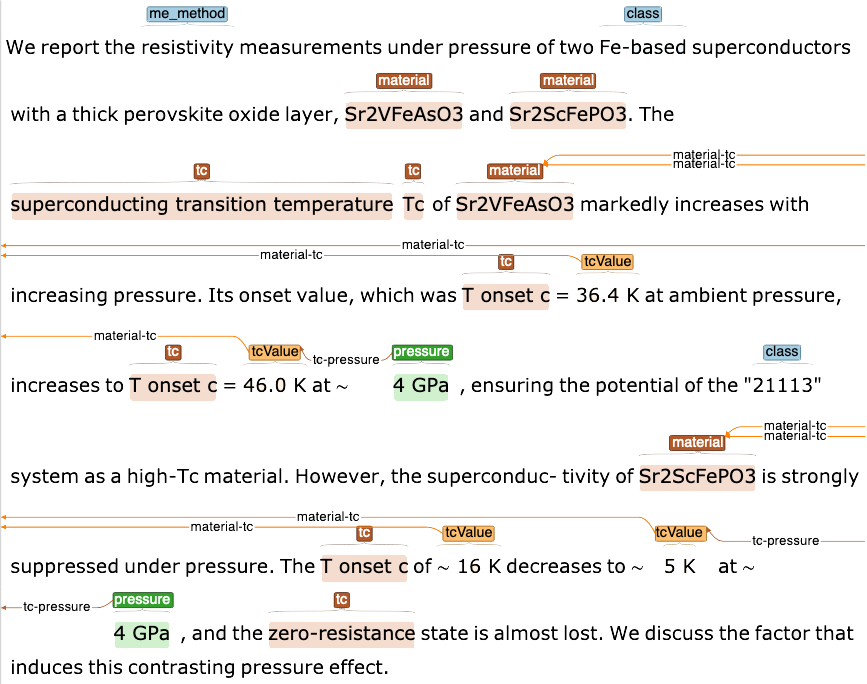
\includegraphics[width=\linewidth]{figures/supermat/Fig1.png}
  \caption{Example in the annotated corpus. Excerpt from © 2009 The Physical Society of Japan (J. Phys. Soc. Jpn. 78, 123707)}
  \label{fig:example-annotations-and-links}
\end{figure}


\subsection{Entities}
Entities (also referred to as Named Entities, mentions, or surface forms) are chunks of texts that represent information of interest, as follows: 

\paragraph{Class} (tag: \texttt{<class>}) represents a group of materials defined by certain characteristics.
Superconducting materials can be classified according to different criteria such as the composition and magnetic properties. 
Among publications collected for this study, the domain experts identified three types of classes based on: (a) the composition and crystal structure, (b) material phenomena (e.g. "I-type" and "II-type superconductivity", "BCS superconductors", "nematic", and "conventional/unconventional superconductivity"), and (c) high/low \tc~value (e.g. "high-tc” superconductors). 

In this work, we only considered the (a) classes, mainly because the material composition and crystal structure do not change with time. For example, a cuprate from 1998 is still called a cuprate today. 
In comparison, many material phenomena used for (b) are not robust enough and can be biased by the viewpoint of the author(s) or research group, or the measurement methods. 
Finally, the definition of "high-tc" superconductors (c) is completely relative; i.e., with the progress of research, materials once considered "high-tc" might not be so anymore.

\paragraph{Material} (tag: \texttt{<material>}) identifies the name of one or more materials. 
This label is used to collect the following types of information: 
\begin{itemize}
    \item Chemical formula indicating the material by its general or stochiometric formula (e.g. \texttt{LaFe\textsubscript{1-x}O\textsubscript{7}}, \texttt{WB\textsubscript{2}}),
    \item Compositional name (e.g. \texttt{magnesium diboride}) or abbreviations (e.g. \texttt{YBCO}), 
    \item The material's shape (e.g. wire, powder, thin film) or form of material (e.g. single/poly crystal), 
    \item Modification by a dopant (\texttt{Zn-doped}, \texttt{Si-doped}) or by percentage of doping (\texttt{2\%-doped}). We also considered qualitative expressions such as \textit{overdoped}, \textit{lightly doped}, and \textit{pure} as valid information, 
    \item Substrate information (e.g. \texttt{grown on MgO(100) film}) when it was adjacent to the material name or formula, in the text,
    \item Additional information about the sample (e.g. \texttt{as-grown}, \texttt{untwinned}, \texttt{single-layer}) when it was adjacent to the material name or formula, in the text. 
\end{itemize}

\paragraph{Superconducting critical temperature} (tag: \texttt{<tc>}) identifies expressions related to the phenomenon of superconductivity. Any temperature mentioned in the text is not necessarily the \tc. Rather, it could refer to the temperature for other processes/events such as annealing/sintering temperature, specific measurements, and structural changes.
This label identifies the presence or absence of superconductivity at a given temperature.
In addition, modifiers of this information (increasing/decreasing \tc) are also retained. 

\paragraph{Superconducting critical temperature value} (tag: \texttt{<tcValue>}) represents the temperature at which the superconducting phenomenon occurs. 
It can be defined by different experimental criteria, such as the onset, mid-point of resistivity drop, or zero resistivity.
This value also considers boundary conditions, such as the \textit{onset of superconductivity}, \textit{zero resistance}. 

\paragraph{Applied pressure} (tag: \texttt{<pressure>}) indicates the applied pressure corresponding to a measured \tc. 

\paragraph{Measurement method} (tag: \texttt{<me\_method>}) indicates the method used to measure or calculate the presence of superconductivity. Here, we considered the following categories: resistivity, magnetic susceptibility, specific heat, and theoretical calculations. 


\subsection{Relations}
\label{relations}
The relations connect entities of materials or samples to their corresponding properties, conditions, and results. 
The connecting links are non-directional, and each entity has no restrictions on the number of links. 
The relation types have been introduced in Section~\ref{subsec:re-solution}.


\subsection{Annotation guidelines}
\label{subsec:annotation-guidelines}
Annotation guidelines include the principles and the rules that describe what constitutes as desired information for the SuperMat dataset and how to annotate it. They include detailed descriptions of the specific rules that have been defined for each type of information to be annotated, with one or more definitions and examples illustrating what to annotate in different cases, exceptions, and references. We used an online system to track the discussions and decisions when a question or a comment was raised and provided a link to such issues in the respective description or example. 
In addition, the guidelines include \textit{linking rules} that provide information on how to connect the entities in a relationship correctly. 
The guidelines were built using a dynamic markup language (called RestructuredText) and stored in a git (\url{https://git-scm.com/}) version control system repository. We deployed them as HTML files via the web, which were updated automatically after each modification. They can be accessed at \url{https://supermat.readthedocs.io}.

\section{Annotation support tools}
\label{subsec:annotation-support-tool}
The task of annotating documents is tedious and requires both attention and subject knowledge from the annotators.
Annotation support tools aim to maximise the efficiency of annotators and minimise human mistakes. 
They comprise a web-based collaborative annotation tool, automatic annotation suggestions, and automatic corpus analysis. 

\subsection{Web-based collaborative annotation tool: INCEpTION}
\label{subsec:annotation-tool}

The annotation tool is the platform used for creating, correcting and linking annotations.
After evaluating several tools, we selected INCEpTION~\cite{tubiblio106270,eckart-de-castilho-etal-2016-web}, a web-based multi-user platform for machine-assisted rapid dataset annotation construction. 
INCEpTION provides supportive functionalities that include: 
\begin{itemize}
    \item Multi-layer annotation sheets allow different annotation schemas over the same documents, 
    \item Two annotation steps: annotation consists of manually correcting pre-imported documents, while curation allows another user to validate the annotations (Figure~\ref{fig:inception-curation-interface}). 
    \item On-the-fly automatic suggestions based on active learning and string matching (Figure~\ref{fig:inception-curation-interface}), 
    \item Bulk annotation corrections, and 
    \item Being open-source (Apache 2.0 license), and under active development at the time of this paper (\url{https://inception-project.github.io/}).
\end{itemize}

\subsection{Annotation suggestions}
\label{subsec:automatic-system-prototype}

Previous works have demonstrated that annotation suggestions improve the quality of the output~\cite{Fort2010InfluenceOP, Nvol2011SemiautomaticSA, Lingren2014EvaluatingTI}.
We provide two types of annotation suggestions. 
(i) \textit{Machine-based annotated data} that were assigned to the documents before loading into the annotation tool. Here, we use a machine learning (ML)-based system from a previously implemented prototype~\cite{foppiano2019proposal} to support our tag-set. 
(ii). \textit{Active learning recommendations} provided by INCEpTION are assigned on the fly based on previous annotations. 
The active-learning recommendations are less precise since they aim to increase the recall, and therefore they need to be explicitly accepted by the annotator.

\subsection{Automatic corpus analysis}
\label{automatic-corpus-analysis}
Automatic corpus analysis is a set of scripts designed to run after the validation step. 
These scripts automatically find inconsistencies in the links and entities, while extracting the statistics of the corpus. 
We calculated the inconsistencies by examining every annotated entity and computing the frequency of the same text being annotated with different labels. 
The script outputs a summary table by visualising each annotation value, as well as their labels and frequencies.
We visually inspected this table because the reported inconsistencies can be either obvious mistakes (Table~\ref{table:dataset-inconsistencies-clear}) or arise from ambiguities (Table~\ref{table:dataset-inconsistencies-unclear}); therefore, their context should be verified. 

\begin{table}[htbp]
    \caption{Statistical overview of the dataset. 
    Links\textsubscript{is} indicates the number of links within the same sentence (intra-sentence). Links\textsubscript{es} indicate the number of links from different paragraphs  (extra-sentence).  }
    \begin{tabular}{ m{6em}   m{4em}  m{6em}  m{7em}  m{6em} } 
    \toprule
        \multirow{2}{5em}{\textbf{Documents}} & \textbf{Files} & \textbf{Paragraphs} &	\textbf{Sentences} & \textbf{Tokens}\\
         & 164  &	2800 & 	20807 & 	1284569\\
    \midrule
        \multirow{2}{5em}{\textbf{Entities}} & \textbf{Entities} &  \multicolumn{2}{|c|}{\textbf{Unique entities}} &  \textbf{ Labels} \\
        & 18698 &  \multicolumn{2}{c}{8071} &  6 \\
    \midrule
        \multirow{2}{5em}{\textbf{Links}} & \textbf{Links} & \multicolumn{2}{|c|}{\textbf{Links\textsubscript{is}}} 
        & \textbf{Links\textsubscript{es}}\\
        & 1524  & \multicolumn{2}{c}{985} &	539	\\
    \bottomrule
    \end{tabular}
    \label{table:summary-content}
\end{table}

Although the links are conceptually non-directed, we have defined a practical convention to maintain their consistency. For example, \textit{material-tcValue} is always represented as a link between \texttt{<tcValue>} and \texttt{<material>} entities. 
The script also computes the statistics (Table \ref{table:summary-content}) for the number of entities (total, unique, by class), the number of links (total, intra- and inter-paragraph, between paragraphs), and other statistical information. 

\begin{table}[htbp]
    \centering\small
    \caption{Inconsistencies resulting from human mistakes.}
     
    \begin{tabular}{ ccccc } 
    \toprule
        Text & Label 1 & \# & Label 2 & \#\\
    \midrule
        \texttt{superconducting transition}     &   \texttt{<material>}   &    1   &   \texttt{<tc>}  &   61   \\
        \texttt{NCCO}    &	\texttt{<material>}   &    14   &   \texttt{<tc>}  &   1   \\
        \texttt{superconducting transition temperatures}     &   \texttt{<material>}   &    1   &   \texttt{<tc>}  &   11   \\
        \texttt{occurrence of superconductivity}    &	\texttt{<material>}   &    1   &   \texttt{<tc>}  &   1   \\
    \bottomrule
    \end{tabular}
    \label{table:dataset-inconsistencies-unclear}
\end{table}

\begin{table}[htbp]
    \centering\small
    \caption{Inconsistencies resulting from the overlapping of \texttt{<material>} and \texttt{<class>} labels.}
    \begin{tabular}{ ccccc } 
    \toprule
        Text & Label 1 & \# & Label 2 & \#\\
    \midrule
        \texttt{LiFeAs}         &   \texttt{<material>}   &    89   &   \texttt{<class>}  &   1   \\
        \texttt{Bi-2212}        &	\texttt{<material>}   &    34   &   \texttt{<class>}  &   1   \\
        \texttt{cobalt oxide}   &   \texttt{<material>}   &    89   &   \texttt{<class>}  &   1   \\
        \texttt{RE-123}         &	\texttt{<material>}   &    34   &   \texttt{<class>}  &   1   \\
    \bottomrule
    \end{tabular}
    \label{table:dataset-inconsistencies-clear}
\end{table}



\section{Annotation process}
\label{subsec:annotation-workflow}
The annotation workflow (Figure~\ref{fig:schema-comparison-modified-workflow}) was designed following the \textit{MATTER} (Model, Annotate, Train, Test, Evaluate, and Revise) schema\cite{pustejovsky2012natural} and other related work~\cite{Dieb2016, Krallinger2015TheCC}.
The workflow is composed of five steps (Figure~\ref{fig:schema-comparison-modified-workflow}): \textit{data-preparation}, \textit{correction}, \textit{validation}, \textit{testing and evaluation}, \textit{revision}. 
This workflow involves three main actors: the automatic process, computer scientists, and the domain experts.


% workflow-schema
\begin{figure}[htbp]
\centering
  \centering
  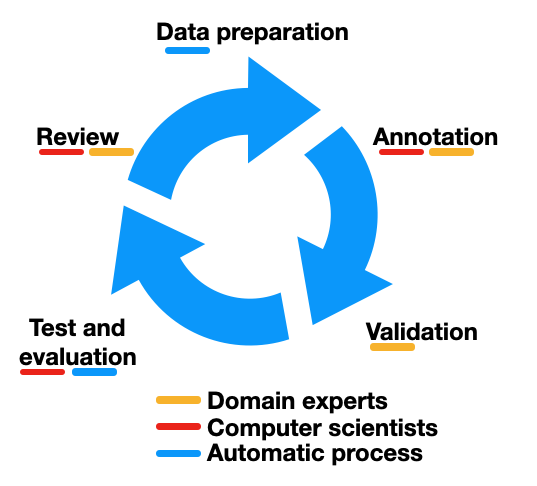
\includegraphics[width=0.5\linewidth]{figures/supermat/Fig2.png}
  \caption{Annotation workflow. Different colours illustrate the involvement of each group at each step of the workflow.}
  \label{fig:schema-comparison-modified-workflow}
\end{figure}

The first step of the annotation process involves preparing the machine-based annotated data from the source PDF documents. 
The PDF files are converted to an XML-based format, and annotation is automatically applied. 
This is followed by four more steps: 

\begin{itemize}
\item Annotation: The human annotator can select a document and manually add, remove, or modify each entity based on rules defined in the guidelines. Once the annotation is complete, the document is marked "ready" for the validation. 

\item Validation/Curation by domain experts: Annotations from different users are validated and merged into a final document (Figure~\ref{fig:inception-curation-interface}). 
The domain expert ("curator"), can compare the different annotated versions, and select the best combination of annotations, or add new ones. 
This step ensures that the annotations are cross-checked and that the document is validated by domain experts.

\item Automatic consistency checks and statistical analysis: This step aims to discover obvious mistakes such as mislabelling or incorrect linking. 
A sequence labelling model is trained and evaluated using 10-fold cross-validation. The evaluation provides precision, recall, and f-score metrics for all the labels.
The resulting model is used for producing machine-based annotated data in the following iteration.

\item Review: Retrospective analysis of the past iteration, where unclear cases are discussed and documented in the annotation guidelines. 

\end{itemize}

\section{Data transformation}
\label{subsec:transformation-of-data}
There are two processes of data transformation (Figure~\ref{fig:data-transformation}): (a) from the source document (PDF) to the dataset format representation (XML-based), and (b) from the dataset format representation to the annotation tool exchange formats (\url{https://inception-project.github.io/releases/0.16.1/docs/user-guide.html\#sect_formats}) and vice-versa. 

\begin{figure}[htbp]
    \centering
    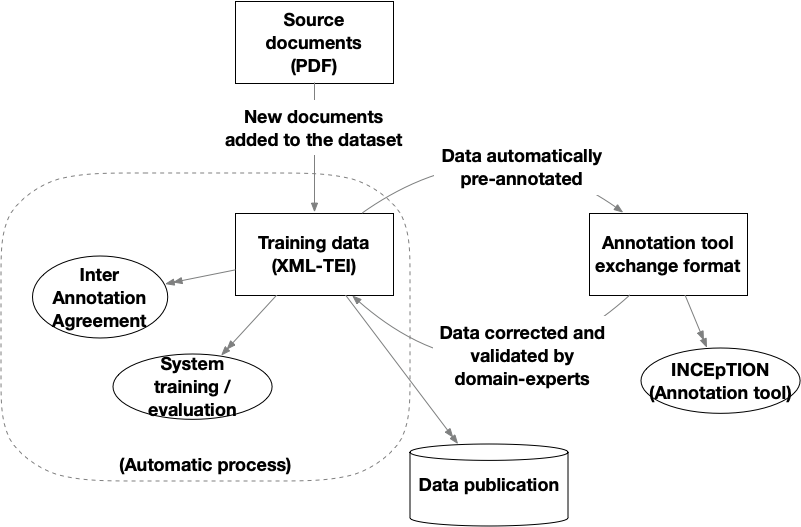
\includegraphics[width=\linewidth]{figures/supermat/Fig3.png}
    \caption{Summary of the data transformation flows.}
    \label{fig:data-transformation}
\end{figure}

\begin{itemize}
    \item PDF to XML-based: This step converts the PDF source document to the dataset format representation in XML following the Text Encoding Initiative (TEI, \url{https://tei-c.org/}) format guidelines. 
    Such transformation is performed by leveraging the functionalities provided by Grobid (\url{https://github.com/kermitt2/grobid}).
    
    We developed a customised process for collecting a subset of information from the source PDF document.
    The process extracts the title, keywords, and abstract from the header; and paragraphs, sections. and figure and table captions from the body.
    All the callouts to references, tables, and figures are ignored.
    The resulting structured document is then encoded in XML as will be described below. 
    \item XML to the annotation tool exchange formats: We transform our XML-formatted data into an INCEpTIONS compatible import format, such as the Webanno TSV 3.2 (\url{https://inception-project.github.io/releases/0.17.0/docs/user-guide.html\#sect_formats_webannotsv3}), and vice-versa using a set of Python scripts. 
    The Webanno TSV 3.2 format is an extension of the CONLL (\url{https://www.signll.org/conll/}) format, with additions of the header and column representation.
\end{itemize}

\section{Data Record}
\label{sec:data-record}
The dataset is composed of 164 PDF documents. Although we used the pre-print version of most of the articles to comply with copyright restrictions, the dataset cannot be distributed and is not publicly available in our repository. 
The three leading publishers represented in the corpus are the American Physical Society (APS), Elsevier, and IOP Publishing (Figure~\ref{fig:distribution-by-publisher}).
Figure~\ref{fig:distribution-by-year} illustrates the distribution by publication date.
We summarise SuperMat's content in Table~\ref{table:summary-content}, with the statistics of documents, entities, and links given separately. In particular, this dataset contains 16052 (7166 unique) entities spread over six labels and 1398 links. 

\begin{figure}[htbp]
\centering
\subfloat[Distribution by publisher.]{\resizebox*{8cm}{!}{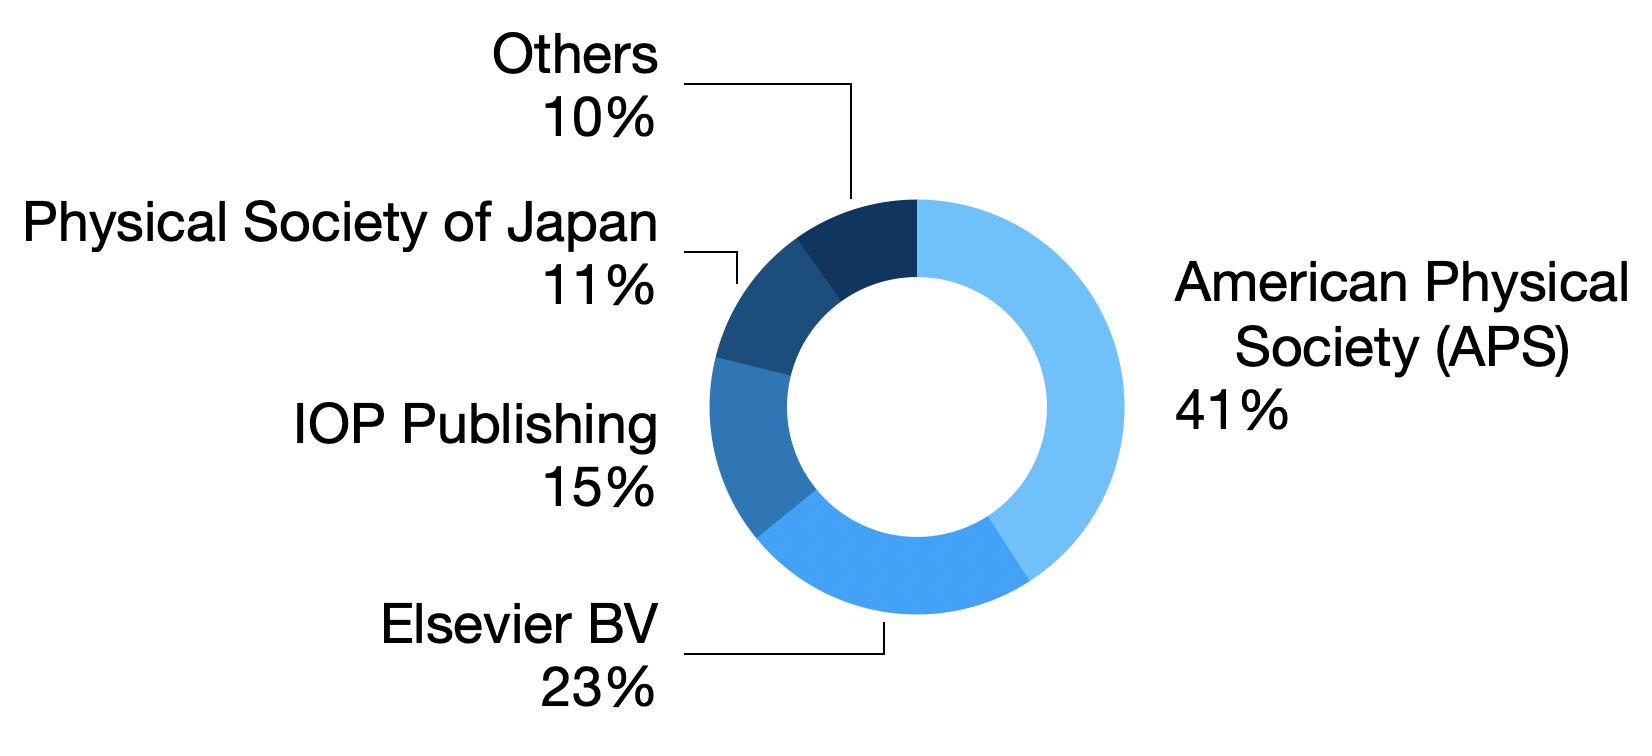
\includegraphics{figures/supermat/Fig5.png}}\label{fig:distribution-by-publisher}} 
\hspace{5pt} 
\subfloat[Distribution by year of publication.]{\resizebox*{6cm}{!}{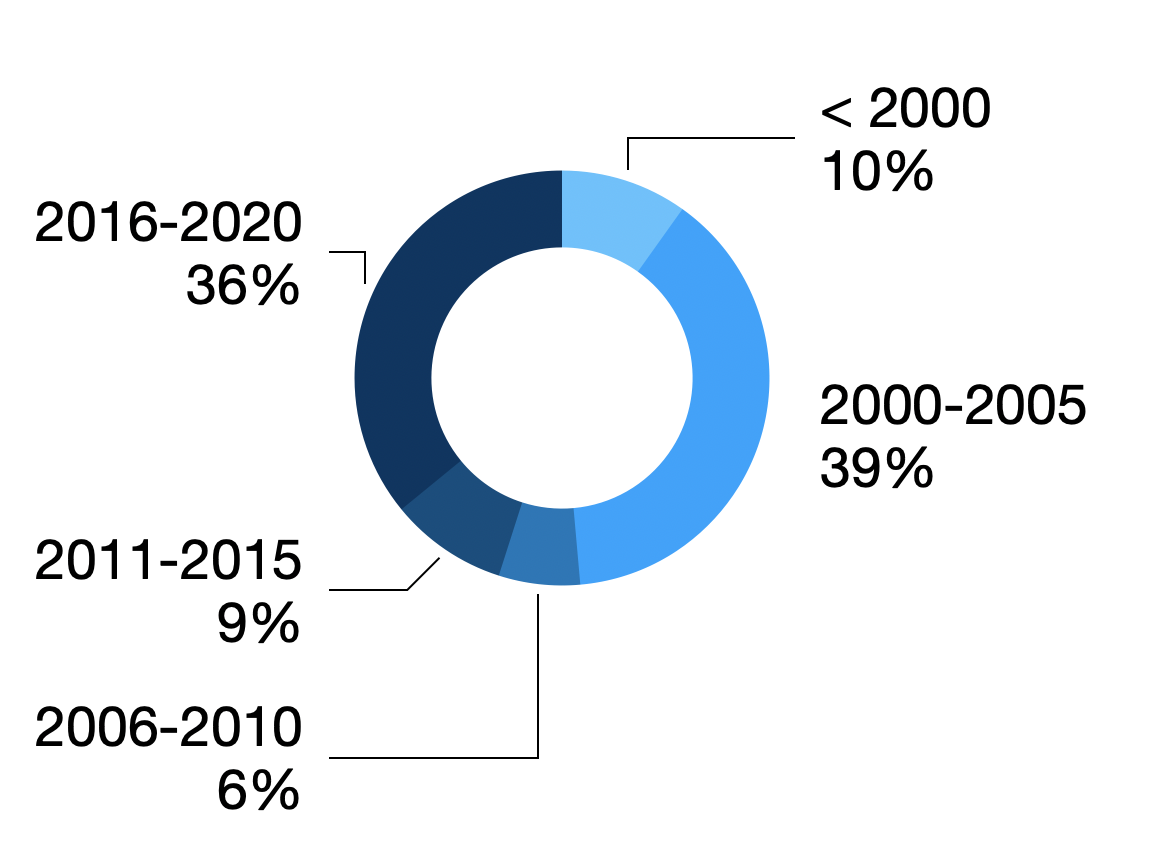
\includegraphics{figures/supermat/Fig6.png}}\label{fig:distribution-by-year}} 
\caption{Distribution of paper in the dataset by (a) publisher, and (b) year of publication.} 
\label{fig:dataset-distributions}
\end{figure}

Each document is encoded according to the XML TEI guidelines, which is a rich format for document representation. 
We have carried out no specific customisation, in order to remain fully compliant with the general TEI schema.
A TEI document has two main parts: the header (within the \texttt{<teiHeader>} tags) containing all the document metadata, and the body (within the section delimited by the \texttt{<text>} tag). 
The transformed data has the following structure: 

\begin{verbatim}
<TEI xml:lang="en" xmlns="http://www.tei-c.org/ns/1.0">
    <teiHeader>
        <fileDesc>
            <titleStmt>
                <title>[...]</title>
            </titleStmt>
            <publicationStmt>
                <publisher>[...]</publisher>
            </publicationStmt>
        </fileDesc>
        <encodingDesc/>
            <abstract>
                <p>[...]</p>
                <ab type="keywords">[...]</ab>
            </abstract>
        <profileDesc>
        </profileDesc>
    </teiHeader>
    <text>
        <body>
            <p>[...]</p>
            <ab type="tableCaption"> [...] </ab>
            <p> [...] </p>
            <ab type="figureCaption"> [...] </ab> 
        </body>
    </text>
</TEI>
\end{verbatim}

We transformed the source documents into these TEI-compliant structures using a simplified representation for specific content types.
The general objective is to flatten the content into a generic structure where priority is given to the annotations.
For instance, the keywords section, which groups together the key terms defined by the author(s) of the paper, is encoded using the generic tag \texttt{<ab type="keywords">} as free text, instead of the dedicated \texttt{<keywords>} element that would typically be part of the header. 
For both the abstract and the article body, the text is segmented in paragraphs (by means of the \texttt{<p>} element). 
The text is annotated with the generic \texttt{<rs>} (referencing string) element adorned with three attributes: \texttt{@type} (the entity type), \texttt{@corresp} (to provide a link to another annotation such as from \textit{material} to \tc~), and \texttt{@xml:id} (to uniquely identify the annotation for referencing or linking purposes).

Because only the captions of tables and figures are retained from the original source, a simplified encoding was defined by means of the \texttt{<ab>} element characterised by a \texttt{@type} attribute; that is, \texttt{<ab type="figureCaption">} for figure captions and \texttt{<ab type="tableCaption">} for table captions. 
Here is an example: 

\begin{verbatim}
<p>
    The electron-doped high-<rs type="tc">transition-
    temperature</rs> (<rs type="tc">Tc</rs>) <rs 
    type="class">iron-based pnictide</rs> 
    superconductor <rs type="material" 
    xml:id="m6">LaFeAsO1-xHx</rs> has a unique 
    phase diagram: Superconducting (SC) double domes are 
    sandwiched by antiferromagnetic phases at ambient 
    pressure and they turn into a single dome with 
    a maximum <rs type="tc">Tc</rs> that 
    <rs type="tcValue" xml:id="m7" 
    corresp="#m6,#9">exceeds 45K</rs> 
    at a pressure of <rs type="pressure" 
    corresp="#m7">3.0 GPa</rs>. 
    [...]
</p>
\end{verbatim}

In the above snippet, the entities \textit{"3.0 GPa"}, \textit{"exceed 45K"} and \textit{"LaFeAsO1-xHx"} are linked together via the pairs \texttt{@corresp, @xml:id}. 
This schema supports multiple annotations to any part of the document. 
For example, the entity \textit{exceed 45K} has a second link with the corresponding identifier (\textit{"\#9"}) to an annotation outside this paragraph.


\section{Practical applications}
The dataset was used in the following practical applications: 

\begin{itemize}
    \item Evaluation tasks: SuperMat has been used for evaluation of Large Language Models (LLM) in mining experimental data. In particular, NER and RE were tested and applied to the materials science literature~\cite{foppiano2024mining}. The dataset not being publicly available counted in a lower chance of being used for pre-training the LLM. 
    \item Automatic extraction: As discussed in Chapter~\ref{cha:extraction-experimental-data}, we used this dataset to develop a system for information extraction for superconducting materials.
    \item Weighted clustering was implemented using SuperMat annotations to identify research papers that discuss specific information of interest in different categories of superconducting materials. The annotations were used to bias the clustering algorithm towards entity similarity to achieve a more targeted clustering toward a specific type of information~\cite{dieb2022superconductor}.
\end{itemize}

\label{sec:technical-validation}
\section{Technical Validation} 
The following measures were employed to ensure the creation of a high-quality dataset: 
\begin{itemize}
    \item Each document was revised and validated by domain experts, 
    \item The workflow begins by assigning machine-based annotated data. This has demonstrated to improve the annotation task over several aspects, namely: time consumption, error rate, and annotation agreement~\cite{Fort2010InfluenceOP,Nvol2011SemiautomaticSA,Lingren2014EvaluatingTI}.
    \item On-the-fly automatic annotation recommendations, which provide fresh suggestions based on online decisions made by the annotators.
    \item The annotators have rapid access to changes in the annotation guidelines.
    \item The discussions were documented and linked in the guidelines. 
    \item Reviews are discussed and approved collaboratively between domain experts and other annotators.
\end{itemize}

\begin{table}[htbp]
    \centering
    \caption{Average IAA between the annotated and validated documents}
    \begin{tabular}{ c|c } 
    \toprule
        \textbf{Label} & \textbf{Average}\\
    \midrule
        \texttt{<material>}     &   0.956   \\
        \texttt{<me\_method>}   &	0.887   \\
        \texttt{<pressure>}     &	0.723   \\
        \texttt{<class>}        &	0.925   \\
        \texttt{<tcValue>}      &	0.863   \\
        \texttt{<tc>}           &	0.831   \\
    \midrule
        \textbf{Micro avg.}     &	0.911	\\
    \bottomrule
    \end{tabular}
    
    \label{table:average-iaa}
\end{table}

These guidelines are a vital piece of this work since they contain knowledge accumulated from these activities.
However, measuring the completeness of the guidelines is challenging. 
Assuming that the documents validated by domain experts represent the ground truth, we conducted IAA analysis between different annotators against the ground truth, using the Krippendorf's Alpha metric~\cite{Krippendorff2004ReliabilityIC}.
Table~\ref{table:average-iaa} shows the average IAA which is satisfying with a value of approximately 0.9. 
The highest score is obtained in the \texttt{<material>} entities, while the lowest one is obtained in \texttt{<pressure>}, which appears less frequently in the papers. 
The disagreement in \texttt{<tcValue>} can appear to be too low as compared with other labels such as \texttt{<class>}, which is, at first look, more ambiguous. 
We analysed the different cases and identified three reasons why this happens. 
First, \texttt{<tcValue>} may depend heavily on the context that requires more human attention, and it is therefore more prone to errors. 
Second, our suggestions system is challenged in its ability to disambiguate critical temperatures from other temperature data, leading to incorrect or invalid suggestions. 
Finally, the presence of mathematical symbols (e.g. "\texttt{\~}", "\texttt{<}", and "\texttt{>}") or other modifiers ("\texttt{up to}", "\texttt{exceeds}", etc.) before the \texttt{<tcValue>} could generate small disagreements that accumulate in the average score. 

\begin{table}[htbp]
    \centering
    \caption{Calculated IAA for annotations produced by domain experts, non-domain experts, and novices compared to the validated version. Annotations from domain experts are cross validated. }
    \begin{tabular}{ ccccc } 
    \toprule
        \textbf{Label} & \textbf{Domain experts} & \textbf{Non-domain experts} & \textbf{Novices}\\
    \midrule
        \texttt{<material>}     &   0.969   & 0.950    &   0.924   \\
        \texttt{<me\_method>}   &   0.890   & 0.862    &   0.901   \\
        \texttt{<pressure>}     &   0.836   & 0.741    &   0.746   \\
        \texttt{<class>}        &   0.990   & 0.836	   &   0.899   \\
        \texttt{<tcValue>}      &   0.895   & 0.734	   &   0.841   \\
        \texttt{<tc>}           &   0.874   & 0.776	   &   0.830   \\
    \midrule
        \textbf{All labels}        &	0.940   &   0.882	&      0.896   \\
    \midrule
        \textbf{\# paragraphs}  &   1066   &  1648	    &   325     \\
    \bottomrule
    \end{tabular}
   
    \label{table:comparison-iaa-nde-de}
\end{table}

To more precisely isolate the impact of the guidelines, we grouped the IAA results by level of domain experience. 
Table~\ref{table:comparison-iaa-nde-de} displays the IAA between the validated data and the data corrected by (a) domain experts (researchers who conduct superconducting development experiments), (b) non-domain-experts (researchers with no experience with superconducting materials), and (c) novices (students in materials science with limited domain experience). 
Obviously, the domain experts have the highest agreement and the IAA value (around 0.95) is 0.06 higher on average than that of non-domain experts. 
Thus, superconducting materials is a complex domain that requires knowledge in materials science to produce high-quality data, while crowdsourcing initiatives such as the Amazon Mechanical Turk might not work well. 

Furthermore, we measured the reliability of the guidelines by observing how quickly novices could reach a satisfying agreement with the validation of the domain experts, without any previous training on the guidelines.
From Table~\ref{table:comparison-iaa-nde-de}, the  novices can attain high IAA results by only using the guidelines and our annotation support tools. 
The average difference in agreement with domain experts (around 0.05) indicates that the guidelines are precise and complete, and that the annotations tools offer sufficient support. 

\section{Data Availability}
\label{sec:code-availability}
The references of the original papers and their bibliographical information, the annotation guidelines sources, and the developed code are available at the GitHub repository \url{https://github.com/lfoppiano/SuperMat}. The guidelines are freely accessible at \url{https://supermat.readthedocs.io}.
The data transformation scripts were written in Python and can be run from the command line. 
They require BeautifulSoup  (\url{https://www.crummy.com/software/BeautifulSoup/}), an open-source library for parsing XML and HTML formats. 
The data analysis scripts were developed as Jupyter notebooks (\url{https://jupyter.org/}) which can easily output results and graphs in the browser. 
The open source annotation tool is INCEpTION (\url{https://inception-project.github.io/}). 
The OA content was acquired using biblio-glutton (\url{https://www.github.com/kermitt2/biblio-glutton}). 
We computed the IAA using the Java library DkPro statistics (\url{https://dkpro.github.io/dkpro-statistics/})~\cite{Meyer2014DKProAA}.

% inception-curation-new.png
\begin{figure}[htbp]
    \centering
    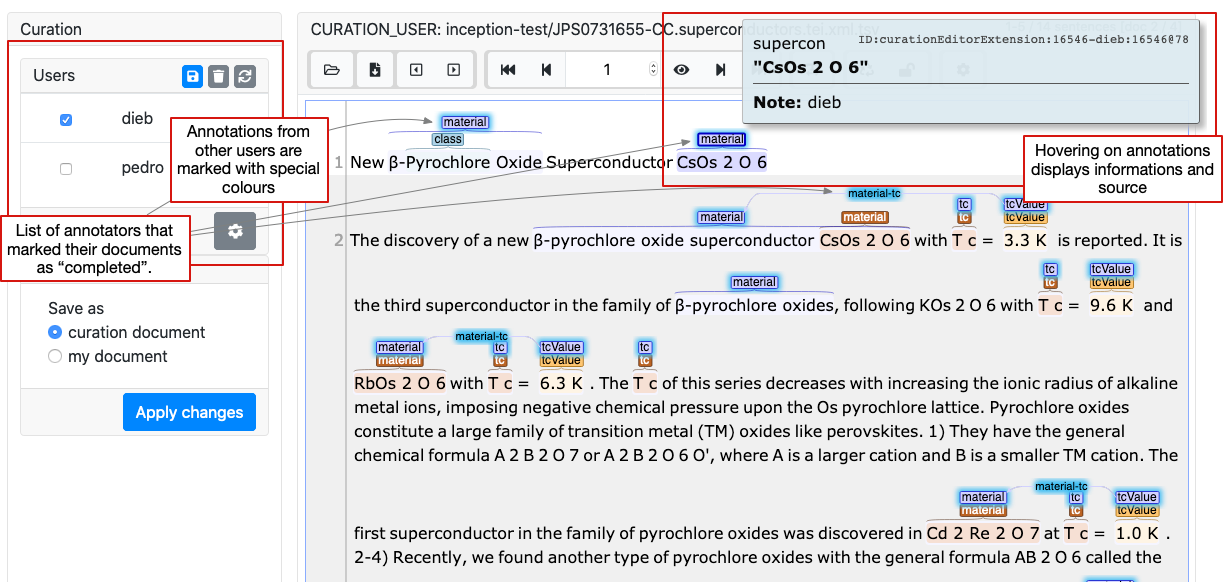
\includegraphics[width=\linewidth]{figures/supermat/Fig7.png}
    \caption{INCEpTION curation interface. Excerpt from © 2004 The Physical Society of Japan (J. Phys. Soc. Jpn. 73, 1655-1656)}
    \label{fig:inception-curation-interface}
\end{figure}


\section{Conclusions}
This chapter presents the process of creating an annotated linked dataset for scientific publications on the development of superconductors. SuperMat aims to create a reliable infrastructure for the improvement of text and data mining processes in the field of superconductor materials. We annotated 164 full-text articles using a two-layer set of annotations. The first layer contains six categories: the names, classes, and properties of materials; links to their respective superconducting critical temperature
(\tc); and parametric conditions such as applied pressure or measurement methods.
The second layer is dedicated to material entities and contains eight classes: formula,
name, doping ratio, etc.
Experts in the field have validated the dataset, which consists of 18698 top-layer entities, with 1524 links between materials, properties, and conditions.
This dataset is the building block for the contribution to material extraction (Chapter~\ref{cha:extraction-experimental-data}) presented in this dissertation. 

This contribution was published in the journal article "SuperMat: Construction of a linked annotated dataset from superconductors-related publications"~\cite{foppiano2021supermat}. 










